\documentclass{article}
\usepackage{natbib}
\usepackage{multirow}
\usepackage{booktabs}
\usepackage{changepage}
\usepackage{caption} % For caption customization
\usepackage{lineno} % For line numbers
\usepackage{graphicx} % For including graphics
% Add line numbers to the document
\usepackage{geometry}


\linespread{1.5} 

\title{Spatio-temporal variability of zooplankton standing stock in eastern Arabian Sea inferred from ADCP backscatter measurements }
\author{Ranjan Kumar Sahu}
\date{\today}
\begin{document}
	
	\maketitle
	\linenumbers
	\section*{Abstract}
	
	The study focuses on the zooplankton standing stock in the eastern Arabian sea (EAS) and aims to understand its spatio-temporal variation using ADCP(acoustic Doppler current profiler) backscatter measurements. The ADCP moorings were deployed at multiple locations on the continental slope of the west coast of India; of which we have used data from October 2017 to January 2023. The ADCP (operating frequency 150 kHz) uses backscatter from or sediments or organisms such as copepods, ctenophores, salps and amphipods greater than 1 cm to calculate current profile. The conversion from backscatter to biomass is based on volumetric zooplankton sampling at the respective locations. Analysis of the data over 25-140 m shows that the backscatter and zooplankton biomass decrease from the upper ocean (215 mg m$^{-3}$ biomass contour) to the lower depths. Seasonal variation is noticed in the monthly climatology zooplankton standing stock (integral of the biomass over the 20-140m water column) along with change as we move to northward slope moorings in EAS. Complementary parameters (mixed layer depth, net primary production, Chl-a, sea surface temperature) is used to explain the processes leading to growth or decay in zooplankton biomass and on their migratory behaviour. Additionally, we have studied the effect of wind induced vertical mixing events. The findings of this research will contribute to a better understanding of the zooplankton dynamics in the EAS and provide valuable insights into the seasonal and annual cycles of zooplankton standing stock.
	
	\newpage
	\section{Introduction}
	\subsection{Background}
	Zooplanktons plays a vital role in food web of pelagic ecosystem by enabling the hierarchical transport of organic matter from primary producers to higher trophic levels impacting the fish population and the carbon pump of the deep ocean (\citep{ohman2001density,le2016global}). They are presumably the largest migrating organisms in terms of biomass (\citep{hays2003review} which happens in Diel Vertical Migration (DVM). Zooplanktons depend not only on phytoplankton but other environmental parameters (e.g. Mixed layer depth, insolation, Oxygen, thermocline, nutrient availability, Chlorophyll concentration and daily primary production). The biological productivity of the ocean is essentially connected with physics and chemistry (\citep{subrahmanyan1959studiespart2, ryther1966primary, qasim1977biological, nair1970primary,banse1995zooplankton,mccreary2009biophysical, vijith2016consequences}). The dynamic ocean results in varying physico-chemical properties, leading to bloom and growth of planktons in favourable conditions. The changes are strongly influenced by the seasonal cycle in the North Indian Ocean (NIO; north of ~5o N of Indian Ocean). The eastern boundary of Arabian Sea contains the West India Coastal Current (WICC; \citep{patil1964hydrography,ramamirtham1965hydrography, banse1968hydrography,shetye1991coastal,mccreary1993numerical, shankar1997dynamics, shetye1998coastal, maheswaran2000upwelling, amol2014observed, chaudhuri2020observed,chaudhuri2021observed}) which reverses seasonally, flowing poleward (equatorward) in November to February (June to September). 
	
	The direct consequence of this reversal is the seasonal cycle of thermocline, oxycline and thickness of mixed Layer Depth (MLD) induced by upwelling favourable conditions in summer and downwelling favourable conditions in winter in eastern Arabian Sea (EAS). Further, the phytoplankton biomass and chlorophyll concentration changes with the season (\citep{subrahmanyan1960studies, banse1968hydrography, levy2007basin, vijith2016consequences}). Upwelling in  summer monsoon leads to maximum chlorophyll growth in the entire EAS (\citep{ banse1968hydrography, banse2000geographical, mccreary2009biophysical, hood2017biogeochemical}). During winter monsoon, the convective mixing induced winter mixed layer (\citep{shetye1992does, madhupratap1996mechanism, levy2007basin, vijith2016consequences, shankar2016inhibition, keerthi2017physical}) results in winter chlorophyll peak in northern EAS (NEAS) while the downwelling Rossby waves modulate chlorophyll along the southern EAS (SEAS) limited to coast and islands (\citep{amol2020modulation}). (For a detailed description on EAS division, please refer figure 1 of \citep{shankar2019role}).
	
	The zooplankton grazing peak is instantaneous with no time delay from peak phytoplankton production (\citep{li2000determines}, but its population growth lags (\citep{rehim2012dynamical, almen2020temperature}) depending on its gestation period and other limiting aspects. While some studies suggest that the peak timing of zooplankton may not change in parallel with phytoplankton blooms (\citep{winder2004climatic}), others indicate that lag exists between primary production and the transfer of energy to higher trophic levels (\citep{brock1992interannual, brock1991phytoplankton}). A recent work (\citep{aparna2022seasonal}) had shown that peak zooplankton population may never occur even with a bloom in phytoplankton such as in SEAS, leading to the collapse of ecological models and succeeding food webs of higher trophic levels.  
	
	The conventional zooplankton measurements, where only few snapshot/s of the event is captured gives an incoherent or incomplete understanding in terms of spatio-temporal variation of mesozooplankton (\citep{ramamurthy1965studies, piontkovski1995spatial, madhupratap1992zooplankton,madhupratap1996lack}) as much information is revealed by later studies (\citep{jyothibabu2010re, vijith2016consequences, shankar2019role, aparna2022seasonal}) using high resolution data. Calibrated acoustic instruments such as Acoustic Doppler Current Profiler (ADCP) along with relevant data can be utilised to understand small scale variability (\citep{nair1999arabian, edvardsen2003assessing, smith2005mesozooplankton, smeti2015spatial, kang2024acoustic}), the complex interplay between the physico-chemical parameters and ecosystem (\citep{jiang2007temporal, potiris2018acoustic, shankar2019role, aparna2022seasonal, nie2023influence}), the zooplankton migration (\citep{ursella2018evidence, ursella2021diel}) and their seasonal to annual variation (\citep{jiang2007temporal, hobbs2021marine,liu2022seasonal, aparna2022seasonal}).
	
	\newpage
	
	
	
	
	
	
	
	
	
	
	
{\footnotesize 	\bibliographystyle{plainnat} % Choose a bibliography style
	\bibliography{bs_citations} % Specify your .bib file
}	
\newpage
\newgeometry{top=1cm, bottom=1cm} 
	
\begin{table}[htbp]

	{\footnotesize

		\captionsetup{justification=justified,font=footnotesize,skip=0.05\baselineskip} % Adjust the spacing above and below the caption
		\caption{\newline
			 ADCP deployment detatils at the locations. The temporal resolution is 1 hour, bin size(vertical resolution) 4 m. All ADCPs are operated at 153.3 kHz. The moorings are at a water column depth of 950 - 1200 m on the continental slope and are serviced on yearly basis according to ship availability. The data }
		\begin{adjustwidth}{0in}{0in} 
			\begin{tabular}{ccccccc}
				
				\toprule
				\multicolumn{1}{c}{}        & \multicolumn{2}{c}{Date}                                       & \multicolumn{2}{c}{Depth}                                                              & &          \\ 
				\midrule
				\multicolumn{1}{c}{\begin{tabular}[c]{@{}c@{}} Station \\ (Position; $^o$E,$^o$N) \end{tabular}} & \multicolumn{1}{c}{Deployment} & \multicolumn{1}{c}{Recovery} & \multicolumn{1}{c}{Ocean} & \multicolumn{1}{c}{ADCP} & \multicolumn{1}{c}{Er} & \multicolumn{1}{c}{Kc} \\
				\midrule
				\multirow{4}{*}{\begin{tabular}[c]{@{}c@{}} Okha\\ (67.47, 22.26)\end{tabular}}         & 01/10/2018                      & 01/12/2019                    & 996                        & 118                       & 37                          , 37                          , 37                          , 36 &                           0.42                        , 0.44                        , 0.42                        , 0.43                        \\
				& 01/12/2019                      & 04/12/2020                    & 1166                       & 312                       & 39                          , 36                          , 38                          , 36                          & 0.42                        , 0.44                        , 0.42                        , 0.43                        \\
				& 04/12/2020                      & 08/03/2022                    & 1021                       & 144                       & 41                          , 37                          , 38                          , 37                          & 0.42                        , 0.44                        , 0.42                        , 0.43                        \\
				& 08/03/2022                      & 01/01/2023                    & 1019                       & 142                       & 37                          , 38                          , 39                          , 36                          & 0.42                        , 0.44                        , 0.42                        , 0.43                        \\
				\midrule
				\multirow{5}{*}{\begin{tabular}[c]{@{}c@{}} Mumbai \\ (69.24, 20.01)\end{tabular}}        & 09/11/2017                      & 29/09/2018                    & 1025                       & 150                       & 36                          , 34                          , 39                          , 42                          & 0.40                        , 0.40                        , 0.40                        , 0.40                        \\
				& 29/09/2018                      & 29/11/2019                    & 1122                       & 125                       & 35                          , 36                          , 39                          , 42                          & 0.40                        , 0.40                        , 0.40                        , 0.40                        \\
				& 29/11/2019                      & 02/12/2020                    & 1143                       & 164                       & 37                          , 34                          , 39                          , 43                          & 0.40                        , 0.40                        , 0.40                        , 0.40                        \\
				& 02/12/2020                      & 06/03/2022                    & 1125                       & 142                       & 36                          , 34                          , 39                          , 42                          & 0.40                        , 0.40                        , 0.40                        , 0.40                        \\
				& 07/03/2022                      & 02/01/2023                    & 1103                       & 158                       & 37                          , 34                          , 40                          , 43                          & 0.40                        , 0.40                        , 0.40                        , 0.40                        \\
				\midrule
				\multirow{5}{*}{\begin{tabular}[c]{@{}c@{}} Jaigarh \\ (71.12, 17.53)\end{tabular}}       & 27/10/2017                      & 27/09/2018                    & 1039                       & 198                       & 32                          , 35                          , 33                          , 32                          & 0.45                        , 0.45                        , 0.45                        , 0.45                        \\
				& 27/09/2018                      & 30/10/2019                    & 1032                       & 164                       & 32                          , 35                          , 33                          , 31                          & 0.45                        , 0.45                        , 0.45                        , 0.45                        \\
				& 03/11/2019                      & 30/11/2020                    & 1142                       & 264                       & 32                          , 36                          , 33                          , 32                          & 0.45                        , 0.45                        , 0.45                        , 0.45                        \\
				& 30/11/2020                      & 05/03/2022                    & 1099                       & 119                       & 33                          , 36                          , 34                          , 32                          & 0.45                        , 0.45                        , 0.45                        , 0.45                        \\
				& 03/04/2022                      & 26/06/2022                    & 1120                       & 136                       & 68                          , 71                          , 69                          , 66                          & 0.45                        , 0.45                        , 0.45                        , 0.45                        \\
				\midrule
				\multirow{5}{*}{\begin{tabular}[c]{@{}c@{}} Goa\\ (72.74, 15.17)\end{tabular}}          & 03/10/2017                      & 25/09/2018                    & 1000                       & 174                       & 35                          , 37                          , 34                          , 35                          & 0.44                        , 0.44                        , 0.40                        , 0.41                        \\
				& 25/09/2018                      & 16/10/2019                    & 969                        & 145                       & 38                          , 36                          , 36                          , 34                          & 0.44                        , 0.44                        , 0.40                        , 0.41                        \\
				& 16/10/2019                      & 29/11/2020                    & 966                        & 143                       & 44                          , 38                          , 36                          , 43                          & 0.44                        , 0.44                        , 0.40                        , 0.41                        \\
				& 29/11/2020                      & 03/03/2022                    & 985                        & 157                       & 35                          , 40                          , 35                          , 38                          & 0.44                        , 0.44                        , 0.40                        , 0.41                        \\
				& 03/03/2022                      & 05/01/2023                    & 984                        & 159                       & 35                          , 38                          , 35                          , 34                          & 0.44                        , 0.44                        , 0.40                        , 0.41                        \\
				\midrule
				\multirow{4}{*}{\begin{tabular}[c]{@{}c@{}} Udupi \\ (74.04, 12.5)\end{tabular}}         & 05/10/2017                      & 06/10/2018                    & 1028                       & 176                       & 44                          , 46                          , 29                          , 35                          & 0.45                        , 0.45                        , 0.45                        , 0.45                        \\
				& 06/10/2018                      & 18/10/2019                    & 1027                       & 179                       & 32                          , 38                          , 30                          , 36                          & 0.45                        , 0.45                        , 0.45                        , 0.45                        \\
				& 18/10/2019                      & 11/12/2020                    & 1018                       & 168                       & 33                          , 37                          , 31                          , 38                          & 0.45                        , 0.45                        , 0.45                        , 0.45                        \\
				& 11/03/2022                      & 06/01/2023                    & 1036                       & 155                       & 31                          , 32                          , 32                          , 33                          & 0.45                        , 0.45                        , 0.45                        , 0.45                        \\
				\midrule
				\multirow{5}{*}{\begin{tabular}[c]{@{}c@{}} Kollam \\ (75.44, 9.05)\end{tabular}}        & 07/10/2017                      & 08/10/2018                    & 1174                       & 200                       & 43                          , 55                          , 45                          , 43                          & 0.49                        , 0.50                        , 0.49                        , 0.50                        \\
				& 08/10/2018                      & 20/10/2019                    & 1160                       & 123                       & 49                          , 62                          , 46                          , 46                          & 0.49                        , 0.50                        , 0.49                        , 0.50                        \\
				& 20/10/2019                      & 13/12/2020                    & 1209                       & 176                       & 52                          , 61                          , 54                          , 55                          & 0.49                        , 0.50                        , 0.49                        , 0.50                        \\
				& 13/12/2020                      & 13/03/2022                    & 1129                       & 91                        & 49                          , 51                          , 46                          , 47                          & 0.49                        , 0.50                        , 0.49                        , 0.50                        \\
				& 13/03/2022                      & 08/01/2023                    & 1149                       & 164                       & 41                          , 48                          , 43                          , 41                          & 0.49                        , 0.50                        , 0.49                        , 0.50                        \\
				\midrule
				\multirow{6}{*}{\begin{tabular}[c]{@{}c@{}} Kanyakumari \\ (77.39,6.96)\end{tabular}}   & 16/11/2016                      & 08/10/2017                    & 1096                       & 252                       & 37                          , 36                          , 37                          , 37                          & 0.42                        , 0.44                        , 0.42                        , 0.43                        \\
				& 08/10/2017                      & 10/10/2018                    & 1055                       & 181                       & 32                          , 34                          , 38                          , 35                          & 0.45                        , 0.45                        , 0.45                        , 0.45                        \\
				& 10/10/2018                      & 22/10/2019                    & 1075                       & 180                       & 36                          , 34                          , 39                          , 36                          & 0.45                        , 0.45                        , 0.45                        , 0.45                        \\
				& 22/10/2019                      & 14/12/2020                    & 1060                       & 167                       & 33                          , 35                          , 36                          , 35                          & 0.45                        , 0.45                        , 0.45                        , 0.45                        \\
				& 14/12/2020                      & 14/03/2022                    & 1184                       & 287                       & 34                          , 36                          , 36                          , 35                          & 0.45                        , 0.45                        , 0.45                        , 0.45                        \\
				& 14/03/2022                      & 10/01/2023                    & 1069                       & 172                       & 33                          , 36                          , 42                          , 36                          & 0.45                        , 0.45                        , 0.45                        , 0.45                       
				\\ 
				\bottomrule
			\end{tabular}
		\end{adjustwidth}
	}
	
	
\end{table}
\restoregeometry

\newpage

\begin{table}[htbp]
	
	{\tiny 
		\captionsetup{justification=justified,font=footnotesize,skip=0.05\baselineskip,width=0.8\textwidth} % Adjust the spacing above and below the caption
		\caption{\newline Volumetric samples of zooplankton of various stations. The tags corresponds to cruise and particular station. The sampling depth range is standardised for later years for bin range of 0-25m, 25-50m, 50-75m, 75-100m, 100-150m}
		\begin{adjustwidth}{0.5in}{0in} 
			\begin{tabular}{ccccccc}
				\toprule
				Sample number & Tag & Lat($^o$N)    & Lon($^o$E)   & Date & Time (IST) & Sampling depth range (m)      \\
				\midrule
				1-3         & G1  & 15.18      & 72.79      & 25 Sep 18                 & 452        & 50–25, 100–50, 150–100        \\
				4-6         & G2  & 15.16      & 72.71      & 25 Sep 18                 & 2108       & 50–25, 100–50, 150–100        \\
				7-10        & G2  & 15.16      & 72.71      & 25 Sep 18                 & 2137       & 40–20, 60–40, 80–60, 100–80   \\
				11-14       & J1  &            &            & 26 Sep 18                 & 2000       & 40–20, 60–40, 80–60, 100–80   \\
				15-17       & J2  &            &            & 27 Sep 18                 & 2000       & 50–25, 100–50, 150–100        \\
				18-21       & J2  &            &            & 27 Sep 18                 & 2100       & 40–20, 60–40, 80–60, 100–80   \\
				22-25       & M1  & 20         & 69.19      & 28 Sep 18                 & 2135       & 40–20, 60–40, 80–60, 100–80   \\
				26-27       & M1  & 20         & 69.19      & 28 Sep 18                 & 2205       & 50–25, 100–50                 \\
				28-29       & M2  & 20.01      & 69.2       & 29 Sep 18                 & 2035       & 50–25, 100–50                 \\
				30-33       & M2  & 20.01      & 69.2       & 29 Sep 18                 & 2057       & 40–20, 60–40, 80–60, 100–80   \\
				34-37       & U1  &            &            & 5 Oct 18                  & 2000       & 40–20, 60–40, 80–60, 100–80   \\
				38-40       & U1  &            &            & 5 Oct 18                  & 2100       & 50–25, 100–50, 150–100        \\
				41-43       & U2  &            &            & 6 Oct 18                  & 2000       & 50–25, 100–50, 150–100        \\
				44-47       & U2  &            &            & 6 Oct 18                  & 2100       & 40–20, 60–40, 80–60, 100–80   \\
				48-51       & K1  & 9.06       & 75.42      & 8 Oct 18                  & 421        & 40–20, 60–40, 80–60, 100–80   \\
				52-54       & K1  & 9.06       & 75.42      & 8 Oct 18                  & 449        & 50–25, 100–50, 150–100        \\
				55-56       & K2  & 9.04       & 75.4       & 8 Oct 18                  & 2027       & 50–25, 100–50                 \\
				57-60       & K2  & 9.04       & 75.4       & 8 Oct 18                  & 2045       & 40–20, 60–40, 80–60, 100–80   \\
				\midrule
				61-64       & G2  & 15.16      & 72.74      & 16 Oct 19                 & 829        & 50–25, 75–50, 100–75, 150–100 \\
				65-67       & G3  & 15.16      & 72.74      & 16 Oct 19                 & 1812       & 50–25, 75–50, 100–75          \\
				68-70       & K2  & 9.02       & 75.42      & 20 Oct 19                 & 840        & 50–25, 75–50, 100–75          \\
				71-74       & K3  & 9.04       & 75.43      & 20 Oct 19                 & 1934       & 50–25, 75–50, 100–75, 150–100 \\
				75-78       & KK1 &            &            & 22 Oct 19                 & 742        & 50–25, 75–50, 100–75, 150–100 \\
				79-82       & KK2 &            &            & 22 Oct 19                 & 1925       & 50–25, 75–50, 100–75, 150–100 \\
				83-86         & J1  &            &            & 30 Oct 19                 & 324        & 50–25, 75–50, 100–75, 150–100 \\
				87-89         & J2  &            &            & 4 Nov 19                  & 946        & 75–50, 100–75, 150–100        \\
				90-92         & M2  & 19.98      & 69.22      & 29 Nov 19                 & 1434       & 50–25, 75–50, 100–75          \\
				93-96         & M3  & 20.01      & 69.23      & 30 Nov 19                 & 958        & 50–25, 75–50, 100–75, 150–100 \\
				97-100        & O1  & 22.24      & 67.49      & 1 Dec 19                  & 937        & 50–25, 75–50, 100–75, 150–100 \\
				101        & O2  & 22.25      & 67.46      & 1 Dec 19                  & 1957       & 150-100                       \\
				\midrule
				102-105       & G3  & 15.68      & 73.22      & 28 Nov 20                 & 930        & 50–25, 75–50, 100–75, 150–100 \\
				105-108       & G4  & 15.32      & 73.22      & 29 Nov 20                 & 1558       & 50–25, 75–50, 100–75, 150–100 \\
				108-110       & J2  & 17.85      & 71.21      & 30 Nov 20                 & 1458       & 75–50, 100–75, 150–100        \\
				111-114       & J3  & 17.91      & 71.21      & 1 Dec 20                  & 1052       & 50–25, 75–50, 100–75, 150–100 \\
				115-118       & M4  & 20.03      & 69.38      & 2 Dec 20                  & 2016       & 50–25, 75–50, 100–75, 150–100 \\
				119.00        & O2  & 22.41      & 67.8       & 4 Dec 20                  & 953        & 150-100                       \\
				120-123       & O3  & 22.41      & 67.79      & 4 Dec 20                  & 2011       & 50–25, 75–50, 100–75, 150–100 \\
				124-127       & K3  & 9.11       & 75.72      & 12 Dec 20                 & 2335       & 50–25, 75–50, 100–75, 150–100 \\
				128-131       & K4  & 9.06       & 75.74      & 13 Dec 20                 & 1507       & 50–25, 75–50, 100–75, 150–100 \\
				132-134       & KK1 & 7.62       & 77.63      & 14 Dec 20                 & 1226       & 50–25, 75–50                  \\
				135-138       & KK2 & 7.62       & 77.63      & 14 Dec 20                 & 2047       & 50–25, 75–50, 100–75, 150–100 \\
				\midrule
				139-142       & G4  & 15.32      & 73.21      & 3 Mar 22                  & 823        & 50–25, 75–50, 100–75, 150–100 \\
				143-146       & G5  & 15.68      & 73.21      & 4 Mar 22                  & 1030       & 50–25, 75–50, 100–75, 150–100 \\
				147-150       & M5  & 19.99      & 69.23      & 7 Mar 22                  & 957        & 50–25, 75–50, 100–75, 150–100 \\
				151-154       & O3  & 22.24      & 67.5       & 8 Mar 22                  & 806        & 50–25, 75–50, 100–75, 150–100 \\
				155-158       & U3  & 12.5       & 74.04      & 12 Mar 22                 & 1156       & 50–25, 75–50, 100–75, 150–100 \\
				159-160       & K4  & 9.04       & 75.42      & 13 Mar 22                 & 1027       & 50–25, 75–50, 100–75          \\
				161-164       & KK3 & 6.97       & 77.4       & 15 Mar 22                 & 1220       & 50–25, 75–50, 100–75, 150–100
				\\ 
				\bottomrule
			\end{tabular}
		\end{adjustwidth}
	}
\end{table}


\newpage
\begin{figure}[htbp]
	\centering
	\includegraphics[width=0.6\textwidth]{/media/scilab/disk_ranjan/works/westcoast_adcp1/figures/map_roi.png} 
	\captionsetup{justification=justified,font=footnotesize,skip=0.05\baselineskip,width=0.4\textwidth}
	\caption{Map showing region of interest. The slope moorings are deployed at ~ 1000 m depth.}
	\label{fig:fig1}
\end{figure}


\begin{figure}[htbp]
	\centering
	\includegraphics[width=0.5\textwidth]{/media/scilab/disk_ranjan/works/westcoast_adcp1/figures/linear_fit_line.png} 
	\captionsetup{justification=justified,font=footnotesize,skip=0.05\baselineskip,width=0.7\textwidth}
	\caption{The linear fit line of Biomass (taken in log of biomass) and Backscatter. The linear fit line is within the error range of previous result of \citep{aparna2022seasonal} onto which latest zooplankton volumetric sample data is added.}
	\label{fig:fig2}
\end{figure}


\newpage


\begin{figure}[htbp]
	\centering
	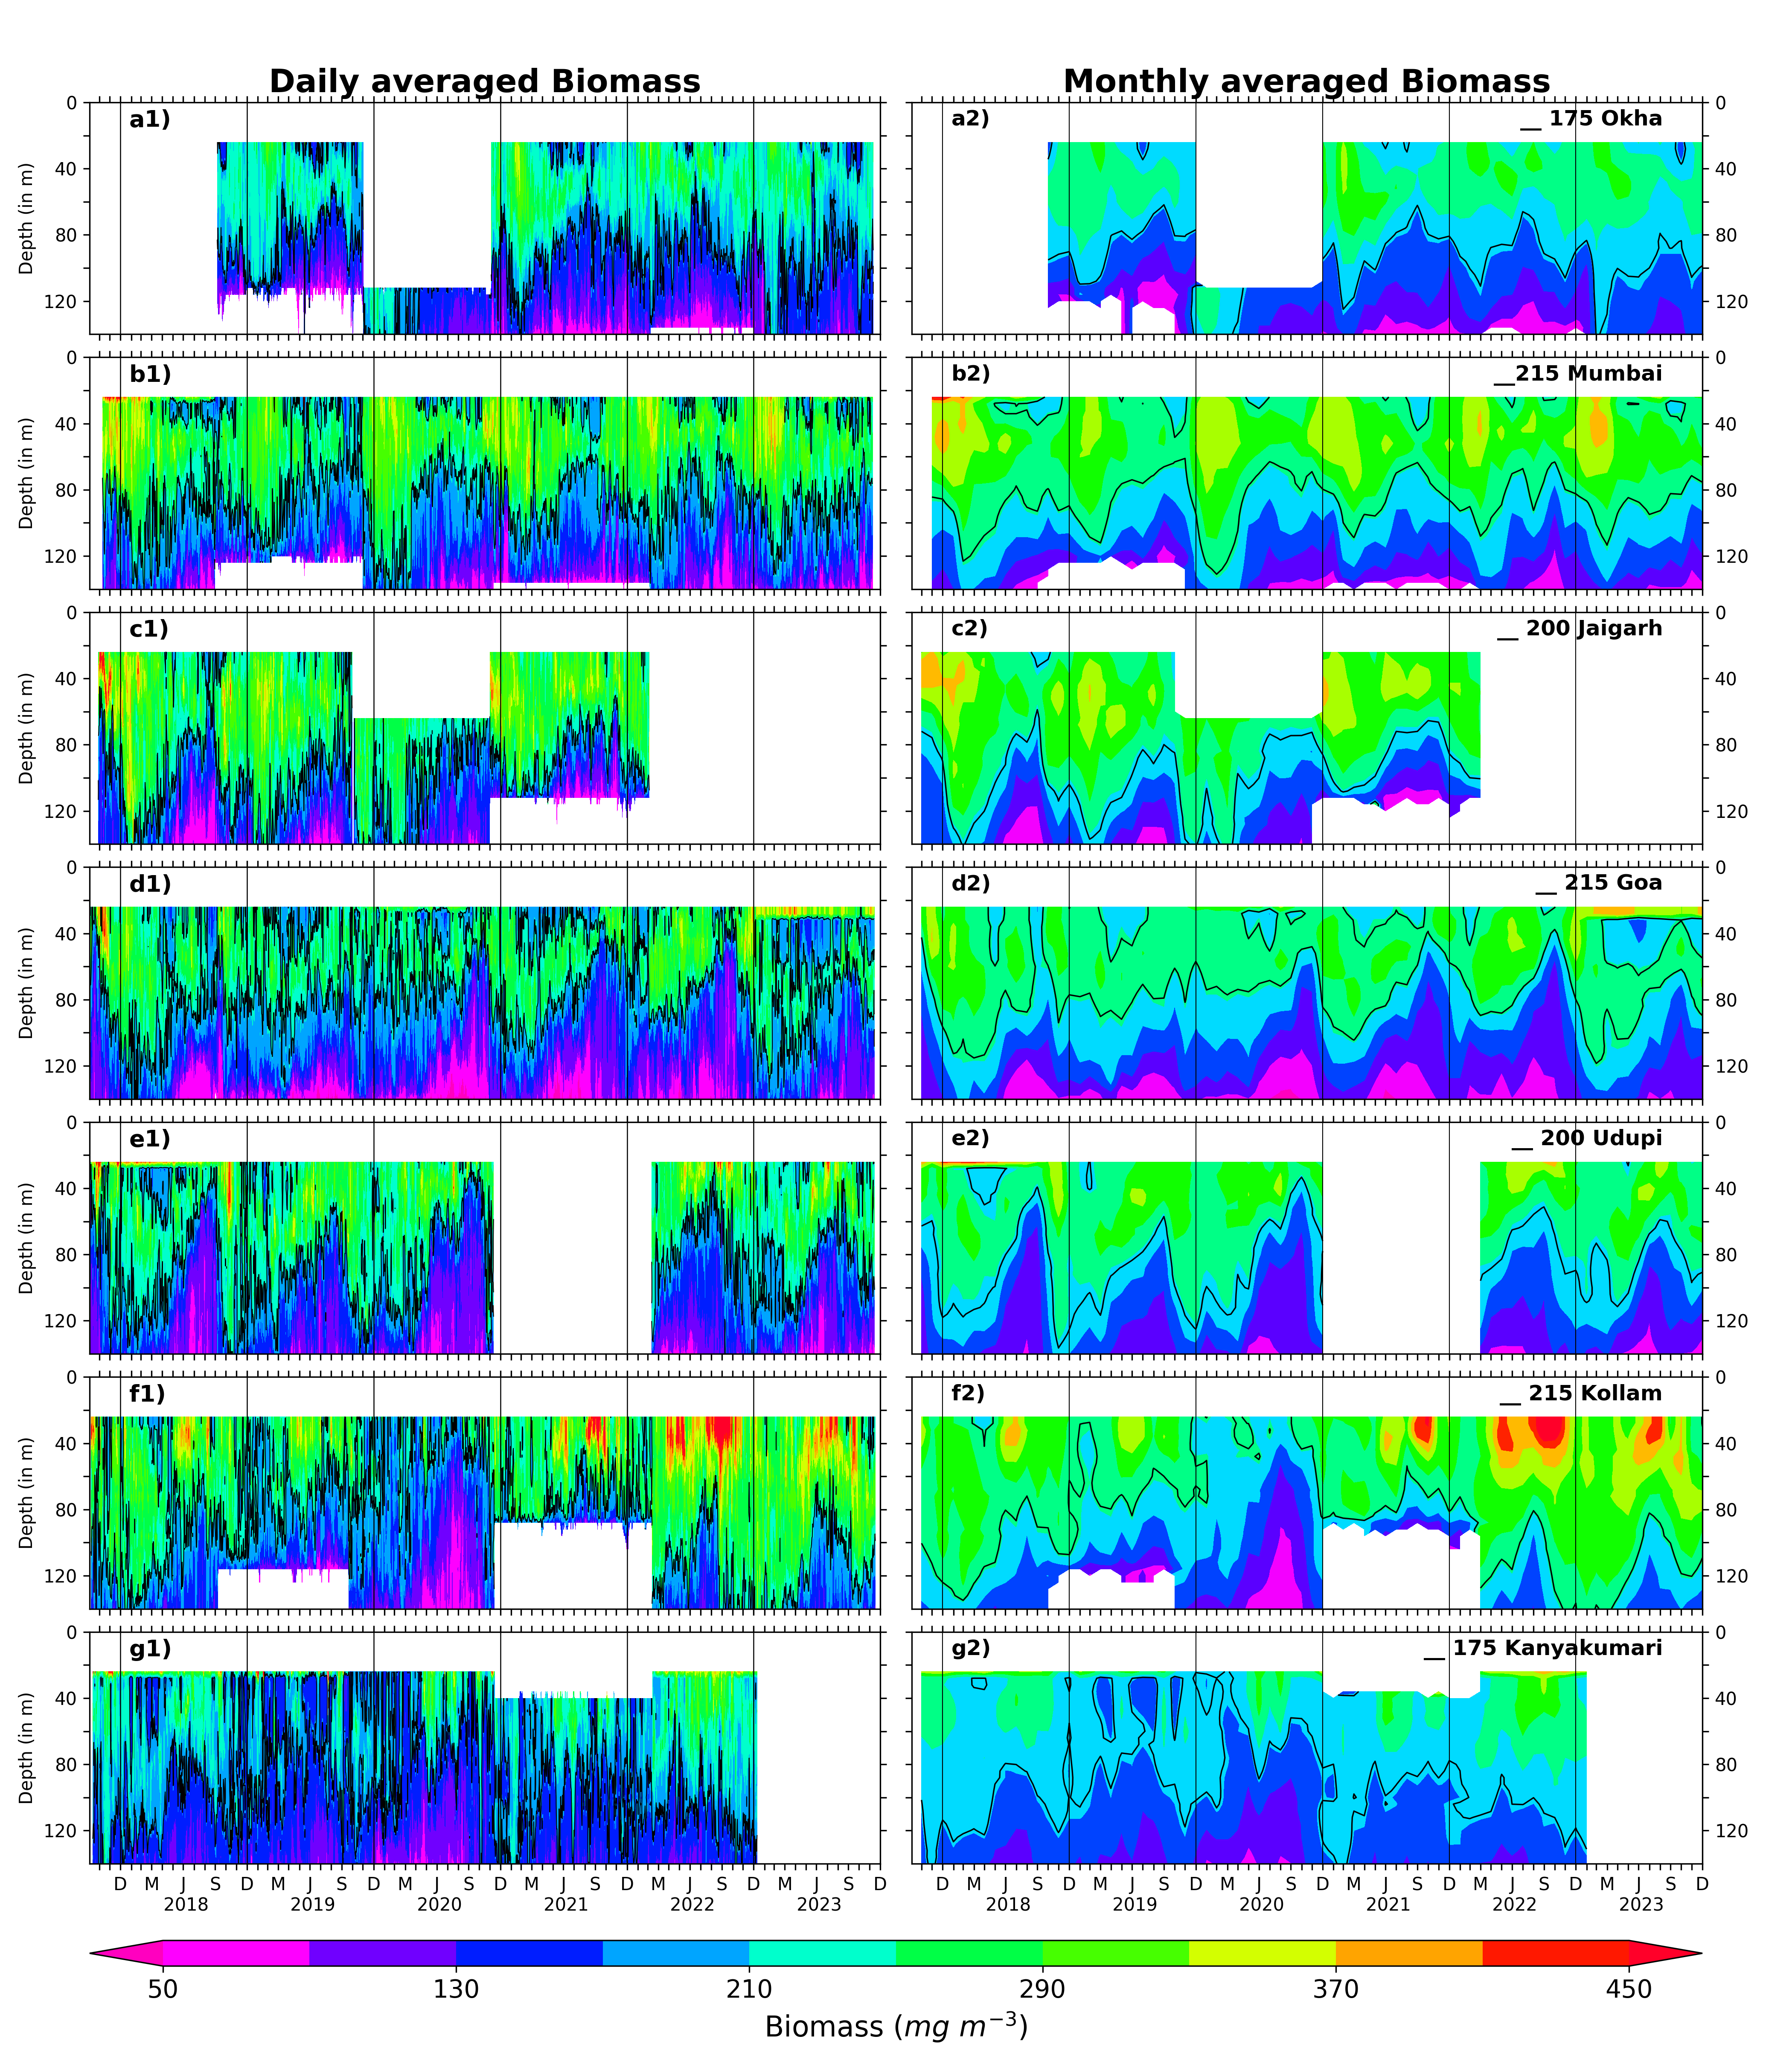
\includegraphics[width=\textwidth]{/media/scilab/disk_ranjan/works/westcoast_adcp1/figures/biomass_daily_monthly.png} 
	\captionsetup{justification=justified,font=footnotesize,skip=0.05\baselineskip,width=\textwidth}
	\caption{The Daily and monthly averaged biomass for EAS moorings, north (top) to south (bottom). The dark contours are marking 215 $mg m^{-3}$.}
	\label{fig:fig3}
\end{figure}



\newpage
\end{document}
